\documentclass[12pt,a4paper]{article}
\usepackage{a4wide}
\usepackage[utf8]{inputenc}
\usepackage[T2A]{fontenc}
\usepackage{graphics,graphicx,epsfig}
\usepackage{amssymb,amsfonts,amsthm,amsmath,mathtext,cite,enumerate,float}
\usepackage[english,russian]{babel}
\usepackage[all]{xy}
\usepackage{morefloats}
\usepackage{pgf}
\usepackage[debug,outputdir={docgraphs/}]{dot2texi}
\usepackage{tikz}
\usepackage{scalefnt}
\usepackage{listings}
\usepackage{float}
\usepackage{verbatim}
\usepackage{placeins}
\usepackage{url}
\usepackage{babelbib}
\usetikzlibrary{shapes,arrows}
\usetikzlibrary{decorations.pathmorphing}

% Comment the following block when compiling this .tex with a saner compiler than texlive.
\makeatletter
\def\@settitle{\begin{center}%
    \baselineskip14\p@\relax
    \bfseries
    \@title
  \end{center}%
}

%\renewcommand{\section}{\@startsection {section}{1}%
%  \z@{.7\linespacing\@plus\linespacing}{.5\linespacing}%
%  {\normalfont}}
\renewcommand{\section}{\@startsection {section}{1}
  \z@{2.7ex \@plus 1ex}{1.0ex}%
  {\normalfont}}
\makeatother

\newtheorem{algo}{Алгоритм}
\newtheorem{theorem}{Теорема}
\newtheorem{stat}{Утверждение}
\newtheorem{defin}{Определение}

\begin{document}
% Comment the following block when compiling this .tex with a saner compiler than texlive.
\pagestyle{plain}
\lstset{language=C++}

\begin{center}
  АЛГОРИТМЫ ПОРОЖДЕНИЯ СУПЕРПОЗИЦИЙ ЭЛЕМЕНТАРНЫХ ФУНКЦИЙ ДЛЯ АППРОКСИМАЦИИ ЭКСПЕРИМЕНТАЛЬНЫХ ДАННЫХ
	\footnote{Работа выполнена при поддержке РФФИ, грант №10-07-00422.}

  \bigskip
  Г.\,И.~Рудой \footnote{Московский физико-технический институт, rudoy@forecsys.ru}
\end{center}

\begin{abstract}
  В~работе
  исследуется алгоритм индуктивного порождения допустимых существенно
  нелинейных моделей. Предлагается алгоритм, порождающий все возможные
  суперпозиции заданной сложности за конечное число шагов, и~приводится его
  теоретическое обоснование. Приводятся результаты вычислительного
  эксперимента, включающего индуктивное порождение набора моделей
  с целью выбора оптимальной модели нелинейной регрессии.

  \bigskip
  \textbf{Ключевые слова}: \emph{символьная регрессия, нелинейные модели, индуктивное порождение,
	сложность моделей.}
\end{abstract}

\section{Введение}

В~ряде приложений \cite{duffy:1999:srised,Barmpalexis201175}
возникает задача восстановления некоторой функциональной зависимости по набору известных данных.
При этом предполагается, что эксперт должен иметь возможность
проинтерпретировать полученную модель в~контексте предметной области.

Одним из методов, позволяющих получать интерпретируемые модели, является
символьная регрессия \cite{davidson:2000:snrea,reference/ml/X10vc,StrijovW10,Strijov08InductMethods},
согласно которой известные данные приближаются некоторой математической
формулой, например, $ \sin x^2 + 2x $ или $\log x - \frac{e^x}{x} $.
Эти формулы являются произвольными суперпозициями функций из некоторого
заданного набора. Одна из возможных реализаций этого метода
предложена Джоном Коза \cite{Koza1998GP, Koza1998Intro}, использовавшим
эволюционные алгоритмы для реализации символьной регрессии. Иван Зелинка
предложил дальнейшее развитие этой идеи \cite{Zelinka2008}, получившее
название аналитического программирования.

Алгоритм построения требуемой математической модели в аналитическом
программировании выглядит следующим образом:
дан набор примитивных функций, из которых можно строить различные формулы
(например, степенная функция, $+$, $\sin$, $\tan$). Начальный набор формул
строится либо произвольным образом, либо на базе некоторых предположений
эксперта. Затем на каждом шаге производится оценка каждой из формул согласно
функции ошибки либо другого функционала качества \cite{Tirsin2005}. На базе
этой оценки у некоторой части формул случайным образом заменяется одна
элементарная функция на другую (например, $\sin$ на $\cos$ или $+$ на
$\times$), а у некоторой другой части происходит взаимный попарный обмен
подвыражениями.

Получаемая формула является математической моделью исследуемого процесса или
явления~--- то есть, это математическое отношение, описывающее основные
закономерности, присущие этому явлению \cite{Pavlovsky2000}.

%DIPLOMA
%Среди возможных путей улучшения качества найденного решения задачи~--- анализ
%информативности различных признаков. Например, в~ходе работы эволюционного
%алгоритма можно выявлять, какие из параметров слабо влияют на качество
%получающейся формулы, и~либо убирать их совсем, либо обеспечивать
%неслучайность замены элементарных функций или обмена поддеревьев с целью
%замены этих параметров на другие в~предположении, что они, возможно,
%окажутся более информативными.

Целью настоящей работы является теоретическое обоснование алгоритмов
индуктивного порождения моделей и~анализ этих алгоритмов. Одним из основных
результатов является доказательство их корректности, то есть, способности
породить искомую формулу.

Алгоритм индуктивного порождения моделей, сформулированный в~настоящей работе,
свободен от некоторых типичных проблем предложенных ранее методов, упомянутых,
например, в~\cite{Zelinka2008}, в том числе:
\begin{itemize}
  \item Порождение рекурсивных суперпозиций, суперпозиций, содержащих
	несоответствующее используемым функциям число аргументов, и~т. д.
	(в~предложенном алгоритме эти проблемы не возникают по построению).
  \item Несовпадение области определения некоторой примитивной функции и области
	значений ее аргументов (возможно, тоже некоторых суперпозиций).
  \item Порождение слишком сложных суперпозиций.
\end{itemize}

Во~второй части работы формально поставлена задача построения алгоритма
индуктивного порождения моделей. Затем, в~третьей части, строится искомый
алгоритм для частного случая беспараметрических моделей и~доказывается его
корректность, а затем алгоритм обобщается на случай моделей, имеющих параметры.
В~четвертой части оценивается количество порожденных предложенным алгоритмом
моделей на каждой итерации. В~пятой части предлагается метод выбора
допустимых моделей из множества всех порожденных моделей. В~шестой части
описываются вспомогательные технические приемы, использованные
в~практическом алгоритме порождения моделей, описанном в~седьмой части. Результаты
вычислительного эксперимента приведены в~восьмой части настоящей работы.

\section{Постановка задачи}

Пусть дана выборка:
\[
D = \{ (\mathbf{x}_i, y_i) \mid i \in \{1, \dots, N\},
			\mathbf{x}_i \in \mathbb{X} \subset \mathbb{R}^n,
			y_i \in \mathbb{Y} \subset \mathbb{R} \},
\]
где $f*$~--- некоторая фиксированная неизвестная функция, $N$~--- число элементов выборки,
$\mathbf{x}_i$~--- вектор значений аргументов функции $f*$ для $i$-ого элемента выборки
(независимых переменных), $y_i$~--- значение функции $f*$ в точке $x_i$ (зависимая переменная),
$\mathbb{X}$~--- множество значений независимых переменных, лежащее в
$\mathbb{R}^n$, $\mathbb{Y}$~--- множество значений зависимой переменной.

Требуется выбрать параметрическую функцию
$f : \Omega \times \mathbb{X} \rightarrow \mathbb{R}$ из
порождаемого множества $\mathcal{F} = \{ f_r \}$, где $\Omega$~--- пространство
параметров, доставляющую минимум некоторому заданному функционалу ошибки $S$.

То есть, для множества всех суперпозиций
\[
\mathcal{F} = \{ f_r \mid
			f_r : (\boldsymbol{\omega}, \mathbf{x}) \mapsto y \in \mathbb{Y},
			r \in \mathbb{N} \},
\]
требуется найти такой индекс $\hat{r}$, что функция $f_r$ среди всех
$f \in \mathcal{F}$ доставляет минимум функционалу качества $S$ при данной
выборке $D$:
\begin{equation}
  \label{eq:hat_r}
  \hat{r} = \arg \min_{r \in \mathbb{N}} S (f_r \mid \boldsymbol{\hat{\omega}_r}, D),
\end{equation}
где $\boldsymbol{\hat{\omega}}_r$~--- оптимальный вектор параметров функции
$f_r$ для каждой $f \in \mathcal{F}$ при данной выборке $D$:
\begin{equation}
  \label{eq:hat_omega}
  \boldsymbol{\hat{\omega}_r} = \arg \min_{\boldsymbol{\omega} \in \Omega} S(\boldsymbol{\omega} \mid f_r, D).
\end{equation}

Сформулируем также постановку теоретической задачи. Для этого сначала
введем понятие суперпозиции функций.

Если множество значений $\mathbb{Y}_i$ функции $f_i$ содержится в области
определения $\mathbb{X}_{i+1}$ функции $f_{i+1}$, то есть
\[
f_i : \mathbb{X}_i \to \mathbb{Y}_i \subset \mathbb{X}_{i+1}, ~~~ i = 1, 2, \dots, \theta - 1,
\]
то функция
\[
f_\theta \circ f_{\theta-1} \circ \dots \circ f_1, ~~~ \theta \geq 2,
\]
определяемая равенством
\[
(f_\theta \circ f_{\theta-1} \circ \dots \circ f_1) (\mathbf{x}) =
  f_{\theta} (f_{\theta-1} (\dots (f_1 (\mathbf{x})))), ~~~ x \in \mathbb{X}_1,
\]
называется \emph{сложной функцией} \cite{MathEnc1984_4} или
\emph{суперпозицией функций} $f_1, f_2, \dots, f_\theta$.

Таким образом, получаем
\begin{defin}
  Суперпозиция функций~--- функция, представленная как композиция нескольких
  функций. 
\end{defin}

Пусть $G = \{ g_1, \dots, g_l \}$~--- множество данных порождающих
функций, а именно, для каждой $g_i \in G$ заданы:
\begin{itemize}
  \item сама функция $g_i$ (например, $\sin$, $\cos$, $\times$),
  \item арность функции и~порядок следования аргументов,
  \item домен ($\text{dom} g_i$) и кодомен ($\text{cod} g_i$) функции,
  \item область определения $\mathcal{D} g_i \subset \text{dom} g_i$ и~область
	значений $\mathcal{E} g_i \subset \text{cod} g_i$.
\end{itemize}
Требуется построить упомянутую функцию $f$ как суперпозицию порождающих
функций из заданного множества $G$.

Поясним различие между последними двумя пунктами. Например, $\text{dom} f$
показывает, значения из какого множества принимает функция $f$ (целые числа,
действительные числа, декартово произведение целых чисел и $\{0, 1\}$,
и~т.~п.). Область определения же показывает, на каких значениях из
$\text{dom} f$ функция $f$ определена и имеет смысл. Так, для функции
$f(x_1, x_2) = \log_{x_1} x_2$:
\[
  \text{dom} f = \mathbb{R} \times \mathbb{R},
\]
\[
  \text{cod} f = \mathbb{R},
\]
\[
  \mathcal{D} f = \{ (x_1, x_2) \mid x_1 \in (0; 1) \cup (1; +\infty), x_2 \in (0; +\infty) \},
\]
\[
  \mathcal{E} f = (-\infty; +\infty).
\]

Требуется также:
\begin{itemize}
  \item построить алгоритм $\mathfrak{A}$, за конечное число итераций
	порождающий любую конечную суперпозицию данных примитивных функций,
  \item указать способ проверки изоморфности двух суперпозиций.
\end{itemize}

Заметим, что мы не требуем для примитивных функций свойства их непорождаемости
в~наиболее общей формулировке типа принципиальной невозможности породить
в~ходе работы искомого алгоритма суперпозицию, изоморфную некоторой функции из
$G$. Такое требование является слишком ограничивающим. В~частности, невозможно
было бы иметь в~$G$ одновременно, например, функции $\text{id}$, $\exp$
и~$\log$, так как $\text{id} \equiv \log \circ \exp$.

В~дальнейшем будем также считать, что суперпозиция, соответствующая
единственной свободной переменной ($f(\mathbf{x}) = x_i$), эквивалентна
функции вида $\text{id} x_i$.

\section{Алгоритм индуктивного порождения допустимых суперпозиций}

%DIPLOMA
\begin{comment}
Введем некоторые понятия из теории графов:

\begin{defin}
  Дерево~--- связный ациклический граф.
\end{defin}

Иными словами, дерево $\Gamma$~--- это некоторый набор вершин $V_i$ и
соединяющих их ребер $E(U, V)$ обладающий следующими свойствами:

\begin{itemize}
  \item Из каждой вершины $V_i$ можно попасть в~каждую другую вершину
	$V_j, j \neq i$ (условие связности).
  \item Для любой вершины $V_i$ не существует пути из нее в~нее же
	(условие ацикличности).
\end{itemize}

\begin{defin}
  Ориентированный граф (орграф)~--- граф, в~котором каждому ребру $E$
  сопоставлено направление.
\end{defin}

Ребра в~орграфах также называются \emph{дугами}.

\begin{defin}
  Ориентированное дерево~--- связный ациклический орграф, в~котором
  только одна вершина не имеет входящих в~нее дуг, а все остальные
  вершины имеют только одну входящую в~них дугу.
\end{defin}

Заметим, что для ориентированного дерева условие связности следует
уточнить. А именно, связность означает, что для любой пары различных
вершин $U$ и~$V$ существует путь между ними без учета направления.

В~дальнейшем мы будем работать в~основном с ориентированными деревьями,
поэтому для краткости будем называть их просто деревьями. В~случае
необходимости неориентированность будет указана явно.

Условимся называть вершину дерева, не имеющую входящих в~нее дуг,
\emph{корнем дерева}:

\begin{defin}
  Корень дерева~--- вершина дерева, в~которую не входит ни одна дуга.
\end{defin}

Условимся обозначать вершину дерева $V_0$.

\begin{defin}
  Лист дерева~--- вершина, из которой не исходит ни одной дуги.
\end{defin}

\begin{defin}
  Уровень вершины~--- длина пути от корня дерева до данной вершины.
\end{defin}

Заметим, что каждой вершине $V_i$ мы можем поставить в~соответствие
поддерево $\Gamma^i$, убрав дугу, приходящую в~$V_i$, и~убрав все вершины,
недостижимые из $V_i$. Корнем такого дерева, очевидно, является $V_i$.

Введем понятия множества смежных вершин для данной вершины:

\begin{defin}
  Множество смежных вершин $S(U)$ для вершины $U$~--- вершины, в~которые
  входит некоторая дуга, выходящая из $U$. Иными словами:
  $S(U) = \{ V \mid \exists E (U, V) \}$.
\end{defin}

Сформулируем алгоритм поиска в~глубину применительно к~ориентированным
деревьям. Будем считать, что вершины одного уровня расположены в~некотором
заранее заданном порядке.

\begin{algo}
  Алгоритм поиска в~глубину (Depth-First Search, $\mathbf{DFS}$).
\end{algo}
\begin{lstlisting}
  map<Vertex, int> DFS (Vertex v, int current)
  {
	map<Vertex, int> result;
	result [v] = current;

	auto children = S (v);

	for (Vertex child : children)
	  result = Unite (result, DFS (child, ++current));

	return result;
  }

  DFS (v0, 0);
\end{lstlisting}

Отметим, что в~общем случае алгоритм $\mathbf{DFS}$ строится более сложным
образом для учета циклов и~случаев несвязных графов.

\begin{figure}[H]
  \begin{tikzpicture}
	\scalefont{2}
	\tikzstyle{n} = [draw, inner sep=2pt, fill=red!20]
	\begin{dot2tex}[dot,options=-tmath,scale=0.5]
	  digraph G1 {
		node [shape="circle",style="n"];
		N1 [label="1"];
		N2 [label="2"];
		N3 [label="3"];
		N4 [label="4"];
		N5 [label="5"];
		N6 [label="6"];
		N7 [label="7"];
		N8 [label="8"];
		N9 [label="9"];

		N1 -> N2;
		N2 -> N3;
		N2 -> N4;
		N1 -> N5;
		N5 -> N6;
		N5 -> N7;
		N7 -> N8;
		N5 -> N9;
	  }
	\end{dot2tex}
  \end{tikzpicture}
  \caption{Порядок обхода вершин при поиске в~глубину}
\end{figure}

\end{comment}

Условимся считать, что каждой суперпозиции $f$ сопоставлено дерево $\Gamma_f$,
эквивалентное этой суперпозиции и~строящееся следующим образом:

\begin{itemize}
  \item В~вершинах $V_i$ дерева $\Gamma_f$ находятся соответствующие
	порождающие функции $g_s, s = s(i)$.
  \item Число дочерних вершин у некоторой вершины $V_i$ равно арности
	соответствующей функции $g_s$.
  \item Порядок смежных некоторой вершине $V_i$ вершин соотвествует порядку
	аргументов соответствующей функции $g_{s(i)}$.
  \item В~листьях дерева $\Gamma_f$ находятся свободные переменные $x_i$
	либо числовые параметры $\omega_i$.
  \item Порядок вершин $V_i$ в~смысле уровня вершин определяет порядок
	вычисления примитивных функций: дерево вычисляется снизу вверх.
	То есть, сначала подставляются конкретные значения свободных переменных,
	затем вычисляются значения в~вершинах, все дочерние вершины которых~---
	свободные переменные, и~так далее до тех пор, пока не останется
	единственная вершина, бывшая корнем дерева. Она и содержит результат
	соответствующего выражения.
\end{itemize}

Таким образом, вычисление значения выражения $f$ в~некоторой точке с данным
вектором параметров $\boldsymbol{\omega} = \{ \omega_1, \omega_2, \dots, \omega_\eta\}$
эквивалентно подстановке соответствующих значений свободных переменных $x_i$
и параметров $\omega_i$ в~дерево $\Gamma_f$, где $x_i$ --- компоненты
вектора признакового описания объекта $\mathbf{x}$.

Заметим важное свойство таких деревьев: каждое поддерево $\Gamma_f^i$
дерева $\Gamma_f$, соответствующее вершине $V_i$, также соответствует
некоторой суперпозиции, являющейся составляющей исходной суперпозиции $f$.

Для примера рассмотрим дерево, соответствующиее суперпозиции
$f = \sin (\ln x_1) + \frac{x_2^3}{2}$ (см. рис \ref{fig:expr_tree_example}).

\begin{figure}[h]
  \centering
  \begin{tikzpicture}
	\scalefont{4}
	\tikzstyle{n} = [draw, inner sep=2pt, fill=red!20]
	  \begin{dot2tex}[dot,options=-tmath,scale=0.4]
		digraph G1 {
		  node [shape="circle",style="n"];
		  
		  Plus [label="\bullet + \bullet"];
		  Sin [label="\sin \bullet"];
		  Ln [label="\ln \bullet"];
		  X1 [label="x_1"];
		  Frac [label="\div"];
		  Pow [label="\bullet^{\bullet}"];
		  X2 [label="x_2"];
		  N3 [label="3"];
		  N2 [label="2"];

		  Plus -> Sin;
		  Sin -> Ln;
		  Ln -> X1;

		  Plus -> Frac;
		  Frac -> Pow;
		  Frac -> N2;

		  Pow -> X2;
		  Pow -> N3;
		}
	  \end{dot2tex}
	\end{tikzpicture}
  \caption{Дерево выражения $\sin (\ln x_1) + \frac{x_2^3}{2}$}
  \label{fig:expr_tree_example}
\end{figure}

Здесь точками обозначены аргументы функций. Как видно, корнем дерева является
вершина, соответствующая операции сложения, которая должна быть выполнена
в~последнюю очередь. Операция сложения имеет два различных поддерева,
соответствующих двум аргументам этой операции. Заметим также, что здесь не
использованы операции типа <<разделить на два>> или <<возвести в~куб>>.
Вместо этого используются операции деления и~возведения в степень в~общем
виде, а в~данном конкретном дереве соответствующие аргументы зафиксированы
соответствующими константами.

\paragraph{Алгоритм порождения суперпозиций.} Сначала определим понятие
\emph{глубины суперпозиции}:

\begin{defin}
  Глубина суперпозиции $f$~--- максимальная глубина дерева $\Gamma_f$.
\end{defin}

Теперь опишем итеративный алгоритм $\mathfrak{A^*}$, порождающий суперпозиции,
не содержащие параметров. Описанный алгоритм породит любую суперпозицию
конечной глубины за конечное число шагов.

Пусть дано множество примитивных функций $G = \{ g_1, \dots, g_l \}$ и
множество свободных переменных $X = \{ x_1, \dots, x_n \}$. Для удобства будем
исходить из предположения, что множество $G$ состоит только из унарных
и~бинарных функций, и~разделим его соответствующим образом на два подмножества:
$G = G_b \cup G_u \mid G_b = \{ g_{b_1}, \dots, g_{b_k} \}, G_u = \{ g_{u_1}, \dots, g_{u_l} \}$,
где $G_b$~--- множество всех бинарных функций, а $G_u$~--- множество всех
унарных функций из $G$. Потребуем также наличия $\text{id}$ в~$G_b$.

\begin{algo}
  Алгоритм $\mathfrak{A^*}$ итеративного порождения суперпозиций.
\end{algo}
\begin{enumerate}
  \item Перед первым шагом зададим начальные значения множества
	$\mathcal{F}_0$ и вспомогательного индексного множества $\mathcal{I}$,
	служащего для запоминания, на какой итерации впервые встречена
	каждая суперпозиция:
	\[
	  \mathcal{F}_0 = X,
	\]
	\[
	  \mathcal{I} = \{ (x, 0) \mid x \in X \}.
	\]
  \item Для множества $\mathcal{F}_i$ построим вспомогательное множество $U_i$,
	состоящее из суперпозиций, полученных в результате применения функций
	$g_u \in G_u$ к~элементам $\mathcal{F}_i$:
	\[
	  U_i = \{ g_u \circ f \mid g_u \in G_u, f \in \mathcal{F}_i \}.
	\]
  \item Аналогичным образом построим вспомогательное множество $B_i$ для
	бинарных функций $g_b \in G_b$:
	\[
	  B_i = \{ g_b \circ (f, h) \mid g_b \in G_b, f, h \in \mathcal{F}_i \}.
	\]
  \item Обозначим $\mathcal{F}_{i+1} = \mathcal{F}_i \cup U_i \cup B_i$.
  \item Для каждой суперпозиции $f$ из $\mathcal{F}_{i+1}$ добавим пару
	$(f, i+1)$ в~множество $\mathcal{I}_f$, если суперпозиция $f$ еще там
	не присутствует.
  \item Перейдем к~следующей итерации, п. 2. 
\end{enumerate}

Тогда $\mathcal{F} = \cup_{i=0}^\infty \mathcal{F}_i$~--- множество всех
возможных суперпозиций конечной длины, которые можно построить из
данного множества примитивных функций.

Вспомогательное множество $\mathcal{I}$ позволяет запоминать, на какой
итерации была впервые встречена каждая суперпозиция. Это необходимо, так
как каждая суперпозиция, впервые порожденная на $i$-ой итерации, будет
порождена также и~на любой итерации после $i$. Одной из возможностей
избежать необходимости в этом множестве является построение
$\mathcal{F}_{i+1}$ как $\mathcal{F}_{i+1} = U_i \cup B_i$ (без
$\mathcal{F}_i$), а множества $U_i$ и $B_i$ строить следующим образом:
\[
  U_i = \{ g_u \circ f \mid g_u \in G_u, f \in \cup_{j=0}^{i} \mathcal{F}_j \},
\]
\[
  B_i = \{ g_b \circ (f, h) \mid g_b \in G_b, f, h \in \cup_{j=0}^{i} \mathcal{F}_j \}.
\]

Алгоритм $\mathfrak{A^*}$ очевидным образом обобщается на случай, когда
множество $G$ содержит функции произвольной (но конечной) арности.
Действительно, для такого обобщения достаточно строить аналогичным образом
вспомогательные множества для этих функций, а именно: для множества функций
$G_n$ арности $n$ построим вспомогательное множество $H_i^n$ вида:
\[
H_i^n = \{ g \circ (f_1, f_2, \dots, f_n) \mid g \in G_n, f_j \in \mathcal{F}_i \}.
\]

В~этих обозначениях $U_i \equiv H_i^1$, а $B_i \equiv H_i^2$.

Тогда множество $\mathcal{F}_{i+1} = \mathcal{F}_i \cup_{n=0}^{n_{max}} H_i^n$,
где $n_{max}$~--- максимальное значение арности функций из $G$.

\begin{theorem}
  Алгоритм $\mathfrak{A^*}$ действительно породит любую конечную суперпозицию
  за конечное число шагов.
\end{theorem}
\begin{proof}
  Чтобы убедиться в~этом, найдем номер итерации, на котором будет порождена
  некоторая произвольная конечная суперпозиция $f$. Чтобы найти этот номер,
  пронумеруем вершины графа $\Gamma_f$ по следующим правилам:
  \begin{itemize}
	\item Если это вершина со свободной переменной, то она имеет номер $0$.
	\item Если вершина $V$ соответствует унарной функции, то она имеет номер
	  $i+1$, где $i$~--- номер дочерней для этой функции вершины.
	\item Если вершина $V$ соответствует бинарной функции, то она имеет номер
	  $i+1$, где $i = \max (l, r)$, а $l$ и $r$ --- номера, соответственно,
	  первой и второй дочерней вершины.
  \end{itemize}

  Нумеруя вершины графа $\Gamma_f$ таким образом, мы получим номер вершины,
  соответствующей корню графа. Это и будет номером итерации, на которой получена
  суперпозиция~$f$.
  
  Иными словами, для любой суперпозиции мы можем указать конкретный номер
  итерации, на котором она будет получена, что и~требовалось.
\end{proof}

В~предложенных ранее методах построения суперпозиций \cite{Zelinka2008}
необходимо было самостоятельно следить за тем, чтобы в~ходе работы алгоритма
не возникало <<зацикленных>> суперпозиций типа $f(x, y) = g (f(x, y), x, y)$.
Заметим, что в~предложенном алгоритме $\mathfrak{A^*}$ такие суперпозиции
не могут возникнуть по построению.

\paragraph{Порождение моделей с параметрами.}
Алгоритм $\mathfrak{A^*}$ в~таком виде не позволяет получать выражения, содержащие численные
параметры $\boldsymbol{\omega}$ суперпозиции $f(\boldsymbol{\omega}, \mathbf{x})$.
Покажем, однако, на примере конструирования множеств $U_i$ и~$B_i$, как
исходный алгоритм $\mathfrak{A^*}$ может быть расширен путем введения параметров:
\[
U_i = { g_u \circ (\alpha f + \beta) },
\]
\[
B_i = { g_b \circ (\alpha f + \beta, \psi h + \phi) }.
\]
Будем обозначать этот расширенный алгоритм как $\mathfrak{A}$. Здесь параметры
$\alpha, \beta$ зависят только от комбинации $g_u, f$ (или $g_b, f, h$ для
$\alpha, \beta, \psi, \phi$). Соответственно, для упрощения их индексы опущены.
Иными словами, мы предполагаем, что каждая суперпозиция из предыдущих итераций
входит в~следующую, будучи умноженной на некоторой коэффициент и~с константной
поправкой.

Очевидно, при таком добавлении параметров $\alpha, \beta, \psi, \phi$
мы не изменяем мощности получившегося множества суперпозиций, поэтому
алгоритм и~выводы из него остаются корректными. В~частности, исходный алгоритм
является частным случаем данного при
$\alpha \equiv \psi \equiv 1, \beta \equiv \phi \equiv 0$.

Переменные $\alpha, \beta, \psi, \phi$ являются параметрами модели. В
практических приложениях можно оптимизировать значения этих параметров у
получившихся суперпозиций, например, алгоритмом Левенберга-Марквардта
\cite{Marquardt1963Algorithm, more:78}.

Заметим также, что такая модификация алгоритма позволяет нам получить единицу,
например, для построения суперпозиций типа $\frac{1}{x}$:
$1 = \alpha\ id\ x + \beta \mid \alpha = 0, \beta = 1$.

Отдельно подчеркнем, что параметры $\boldsymbol{\omega}$ у различных
суперпозиций различны. Однако, так как каждый из параметров зависит только
от соответствующей комбинации функций, к которым он относится, конкретные
значения параметров не учитываются при поиске одинаковых суперпозиций.
Иными словами, при тестировании суперпозиций на равенство сравниваются лишь
структуры соответствующих им деревьев и значения в узлах, соответствующих
функциям и свободным переменным.

Заметим, что и~этот алгоритм очевидным образом обобщается на случай
множества $G$, содержащего функции произвольной арности.

\section{Количество возможных суперпозиций}

Оценим количество суперпозиций, получаемых после каждой итерации алгоритма
$\mathfrak{A}$. Очевидно, с учетом вышеупомянутых оговорок касательно сравнения
параметризованных суперпозиций, это количество равно количеству для алгоритма
$\mathfrak{A^*}$.

Итак, пусть дано $n$ независимых переменных: $| X | = n$, а мощность
множества $G$ распишем через мощности его подмножеств функций соответствующей
арности: $| G_1 | = l_1, | G_2 | = l_2, \dots, | G_p | = l_p$. На нулевой
итерации имеем $P_0 = n$ суперпозиций.

На первой итерации дополнительно порождается:
\[
P_1 = l_1 n + l_2 n^2 + \dots + l_n n^p = \sum_{i=1}^p l_i P_0^i,
\]
и суммарное число суперпозиций после первой итерации:
\[
\hat{P}_1 = P_1 + P_0 = \sum_{i=1}^p l_i P_0^i + P_0.
\]

Как было замечено ранее, суперпозиции, порожденные на $k$-ой итерации, будут
также порождены и~на любой следующей после $k$ итерации, поэтому суммарное
число суперпозиций после второй итерации будет равно:
\[
\hat{P}_2 = \sum_{i=1}^p l_i \hat{P}_1^i.
\]

И вообще, после $k$-ой итерации будет порождено:
\[
\hat{P}_k = \sum_{j=1}^p l_i \hat{P}_{k-1}^i.
\]

Оценим порядок роста количества функций, порожденных после $k$-ой итерации.

\begin{theorem}
  Пусть в множестве примитивных функций $G$ содержится $l_p$ функций арности
  $p > 1$ и ни одной функции арности $p + k \mid k > 0$, и имеется $n > 1$
  независимых переменных. Тогда справедлива следующая оценка количества
  суперпозиций, порожденных алгоритмом $\mathfrak{A}$ после $k$-ой итерации:
  \[
  | \mathcal{F}_k | = \mathcal{O} (l_p^{\sum_{i=0}^{k-1} p^i} n^{p^k}).
  \]
\end{theorem}
\begin{proof}
  Оценим сначала порядок роста для случая, когда есть лишь одна $m$-арная
  функция и~$n$ свободных переменных.

  После первой итерации алгоритма будет порождено $n^m + n$ суперпозиций.
  После второй~--- $(n^m + n)^m + n^m + n$, что можно оценить как 
  $(n^m)^m = n^{m^2}$. И вообще, после $k$-ой итерации количество
  суперпозиций можно оценить как $n^{m^k}$.

  Видно, что для оценки скорости роста количества порожденных суперпозиций
  можно учитывать только функции с наибольшей арностью.

  Рассмотрим теперь случай, когда имеется не одна функция арности $m$, а
  $l_m$ таких функций. Тогда на первой итерации порождается $l_m n^m + n$
  суперпозиций, на второй:
  \[
  l_m (l_m n^m + n)^m + l_m n^m + n \approx l_m^{m+1} n^{m^2},
  \]
  на третьей, с учетом этого приближения:
  \[
  l_m (l_m^{m+1} n^{m^2})^m = l_m l_m^{m(m+1)} n^{m^3} = l_m^{m^2 + m + 1} n^{m^3}.
  \]
  И вообще, скорость роста количества порожденных суперпозиций можно оценить
  как:
  \[
  | \mathcal{F}_k | = \mathcal{O} (l_m^{\sum_{i=0}^{k-1} m^i} n^{m^k}).
  \]
  Таким образом, получаем оценку в общем случае, когда в множестве $G$ содержится
  $l_p$ функций арности $p$ и ни одной функции арности $p + k \mid k > 0$:
  \[
  | \mathcal{F}_k | = \mathcal{O} (l_p^{\sum_{i=0}^{k-1} p^i} n^{p^k}).
  \]
\end{proof}

\section{Множество допустимых суперпозиций}

Предложенный выше алгоритм позволяет получить действительно все возможные
суперпозиции, однако, не все они будут пригодны в~практических приложениях:
например, $\ln x$ имеет смысл только при $x > 0$, а $\frac{x}{0}$ не имеет
смысла вообще никогда. Выражения типа $\frac{x}{\sin x}$ имеют смысл только
при $x \neq \pi k$.

Таким образом, необходимо введение понятия множества \emph{допустимых}
суперпозиций~--- то есть, таких суперпозиций, которые в~условиях данной
задачи корректны.

\begin{defin}
  Допустимая суперпозиция $f$~--- такая суперпозиция, значение которой
  определено для любой комбинации значений свободных переменных, область
  значений $\mathbb{X}$ которых определяется конкретной задачей,
  $\mathbb{X} \subset \mathbb{R}^n$ где $n$~--- число свободных переменных.
\end{defin}

Одним из способов построения только допустимых суперпозиций является
модификация предложенного алгоритма таким образом, чтобы отслеживать
совместность областей определения и~областей значения соответствующих
функций в~ходе построения суперпозиций. Для свободных переменных это,
в свою очередь, означает необходимость задания областей значений
$\mathbb{X}$ пользователем при решении конкретных задач.

Заметим, что, хотя теоретически возможно выводить допустимость выражений
вида $\frac{x}{\sin x}$ исходя из заданных условий на свободную переменную
(например, что $x \in (\frac{\pi}{4}, \frac{\pi}{2})$), в~общем случае это
потребует решения неравенств в~общем виде, что вычислительно неэффективно.

Таким образом, можно сформулировать очевидное \emph{достаточное условие
недопустимости} суперпозиции:

\begin{defin}
  \label{defin:suff_not_allowed}
  Достаточное условие недопустимости суперпозиции $f$: в~соответствующем дереве
  $\Gamma_f$ хотя бы одна вершина $V_i$ имеет хотя бы одну дочернюю вершину
  $V_j$ такую, что область значений функции $g_{s(j)}$ шире, чем область
  определения функции $g_{s(i)}$:
  \[
  \exists i, j : V_i \in \Gamma_f, V_j \in \Gamma_f \wedge \exists \kappa :
	\kappa \in \mathcal{E} g_{s(j)} \wedge \kappa \notin \mathcal{D} g_{s(i)}.
  \]
\end{defin}

Говоря, что область значений функции $f$ шире области определения функции
$g$, мы имеем ввиду, что существует по крайней мере одно значение функции
$f$, не входящее в область определения функции $g$.

Подчеркнем, что, хотя свободные переменные могут принимать, например, все
значения из $\mathbb{R}$, выбором множества $\mathbb{X}$ можно обеспечить
возможность использования их в качестве аргументов функций с более узкой,
чем $\mathbb{R}$, но не менее узкой, чем $\mathbb{X}$, областью определения,
если это не противоречит данной выборке.

Для построения множества допустимых суперпозиций достаточно построить
множество всех возможных суперпозиций при помощи алгоритма $\mathfrak{A}$,
а затем удалить из этого множества все суперпозиции, не удовлетворяющие
сформулированному признаку.

% DIPLOMA
\begin{comment}
\subsection{Множество <<минимальных>> суперпозиций}

В~ходе работы алгоритма могут возникать суперпозиции вида $x + x$ и~$2x$,
и хотя эти выражения эквивалентны, они представляются различными формулами.
Аналогично эквивалентны $x + y$ и~$y + x$, отличающиеся порядком следования
слагаемых. Таким образом, необходим способ нормализации суперпозиций.

Во-первых, необходимо обеспечивать одинаковый порядок следования операндов,
например, упорядочивая их каким-либо образом у коммутирующих бинарных функций.

Во-вторых, необходимо иметь набор правил, позволяющих проверить равенство
$x + x$ и~$2x$. Иными словами, необходимо иметь набор связей между различными
функциями из множества данных примитивных функций. Заметим, что в~общем
случае эта задача требует введения значительного числа правил и~по определению
сводится к~последовательному переборному их применению к~различным
подвыражениям суперпозиции.

В~связи с этим может оказаться более эффективным иной подход к~сравнению
суперпозиций: так как по условию практической задачи значения искомой функции
даны в~конечном числе точек, то для проверки на равенство достаточно вычислить
получившиеся суперпозиции в~этих точках и~сравнить их.

Другим способом, позволяющим избежать разрастания количества правил, может
являться использование только <<независимых>> функций. Например, $\sin$ и
$\cos$ связаны известным тригонометрическим соотношением с точностью до знака,
а значит, $\sin$ и~$\tan = \frac{\sin}{\cos}$ также связаны, как и~ряд прочих
тригонометрических функций, поэтому предлагается среди примитивных функций
оставить лишь $\sin$ и~стандартные арифметические действия для вывода прочих
тригонометрических функций через соответствующие соотношения.

Однако, можно заметить два часто встречающихся шаблона правил, связывающих
различные функции:
\begin{itemize}
  \item Для унарных функций это $f \circ g = h$ (например,
	$\ln \circ \exp = id$).
  \item Для бинарных функций это $ f (x, g (x, i)) = g (x, s (i)) $.
	Например, $x + xi = x(i+1)$: здесь $f = (+), g = (\times), s(i) = i + 1$.
\end{itemize}

В~практических приложениях представляется целесообразным использование
набора правил такого вида вкупе с использованием только <<независимых>>
тригонометрических функций, то есть, по факту, какой-нибудь одной из них
и еще одной обратной.
\end{comment}

\begin{comment}
\subsection{Применимость в задачах классификации} 
Предложенный алгоритм $\mathfrak{A}$ может быть применен и для решения
задач классификации.

Выделим подмножества $G_\mu \subset G$, соответствующие различным дискретным
$\text{cod}$:
$g \in G$:
\[
  G_\mu = \{ g \mid \text{cod} g = \mathbb{Y}_\mu \},
\]
где $\mathbb{Y}_\mu$~--- различные дискретные множества, соответствующие
различным наборам классов.

Тогда суперпозиции, область значений которых соответствует $\mathbb{Y}_\mu$
при фиксированном $\mu$, и являются порожденными алгоритмом $\mathfrak{A}$
классификаторами для класса $\mathbb{Y}_\mu$. Таким образом, достаточно отобрать
из всех порожденных суперпозиций $f$ те, которые имеют в корневой вершине
дерева $\Gamma_f$ функцию $g \in G_\mu$.
\end{comment}

\section{Алгоритм итеративного стохастического порождения суперпозиций}

Несмотря на то, что построенный ранее итеративный алгоритм $\mathfrak{A}$ порождения
суперпозиций позволяет получить за конечное число шагов произвольную
суперпозицию, для практических применений он непригоден в~связи с чрезмерной
вычислительной сложностью, как и~любой алгоритм, реализующий полный перебор.
Вместо него предлагается использовать стохастические алгоритмы и~ряд эвристик,
позволяющих на практике получать за приемлемое время результаты,
удовлетворяющие заранее заданным условиям. В~данном разделе описывается
практически реализуемый вариант алгоритма $\mathfrak{A}$, который и был использован
в~вычислительном эксперименте.

Сначала опишем вспомогательный алгоритм случайного порождения суперпозиции:

\begin{algo}
  \label{algo:RF}
  Алгоритм случайного порождения суперпозиции $\mathcal{RF}$.

  Вход:
  \begin{itemize}
	\item Набор пороговых значений $0 < \xi_1 < \xi_2 < \xi_3 < 1$.
	\item Максимальная глубина порождаемой суперпозиции $Td$.
  \end{itemize}
\end{algo}

Алгоритм работает следующим образом. Генерируется случайное число $\xi$ на
интервале $(0; 1)$, и рассматриваются следующие случаи:
\begin{itemize}
  \item $\xi \leq \xi_1$: результатом алгоритма является некоторая случайно
	выбранная свободная переменная.
  \item $\xi_1 < \xi \leq \xi_2$: результатом алгоритма является	числовой
	параметр.
  \item $\xi_2 < \xi \leq \xi_3$: результатом алгоритма является некоторая
	случайно выбранная унарная функция, для определения аргумента которой
	данный алгоритм рекурсивно запускается еще раз.
  \item $\xi_3 < \xi$: результатом алгоритма является некоторая случайно
	выбранная бинарная функция, аргументы которой порождаются аналогичным
	образом.
\end{itemize}

При этом порождение тривиальных суперпозиций (свободных переменных и
параметров) запрещено: на самом первом шаге пороговые значения масштабируются
таким образом, чтобы всегда порождалась унарная или бинарная функция.
Аналогично при превышении значения $Td$ пороговые значения масштабируются
таким образом, чтобы был порожден узел, соответствующий свободной переменной
или параметру, и алгоритм завершился.

В~ходе работы предлагаемого алгоритма каждой суперпозиции $f$ ставится в
соответствие ее \emph{качество} $Q_f$ (будем также говорить, что
суперпозиция \emph{оценивается}), рассчитываемое исходя из функции ошибки
$S_f$ этой суперпозиции на выборке $D$ и ее сложности $C_f$~---
числа узлов в соответствующем графе $\Gamma_f$, по следующей формуле:
\begin{equation}
  \label{eq:q_f}
  Q_f = \frac{1}{1 + S_f} \left(\alpha \hat{Q} + \frac{1 - \alpha \hat{Q}}{1 + \text{exp} (C_f - \tau)}\right),
\end{equation}
где $\hat{Q}$~--- минимальная приспособленность суперпозиции из критерия
останова, $\alpha$~--- некоторый коэффициент, $0 \ll \alpha < 1$, а
$\tau$~--- коэффициент, характеризующий желаемую сложность модели.
Второй множитель в \eqref{eq:q_f} выполняет роль штрафа за слишком
большую сложность суперпозиции, что подавляет эффект переобучения.

Таким образом, чем лучше результаты суперпозиции, тем ближе значение ее
приспособленности к~$1$, и, наоборот, чем хуже~--- тем ближе к~$0$.

Итак, теперь опишем сам алгоритм:
\begin{algo}
  \label{algo:SA}
  Итеративный алгоритм стохастического порождения суперпозиций.

  Вход:
  \begin{itemize}
	\item Множество порождающих функций $G$, состоящее только из унарных
	  и бинарных функций.
	\item Регрессионная выборка $D$.
	\item $N_{max}$~--- максимальное число одновременно рассматриваемых
	  суперпозиций.
	\item $I_{max}$~--- максимальное число итераций алгоритма.
	\item $\gamma_{mut}$~--- доля суперпозиций, подверженных случайной
	  замене узлов их деревьев.
	\item $\gamma_{cross}$~--- доля суперпозиций, для которых выполняется
	  случайный обмен поддеревьями.
	\item Прочие параметры, используемые в \eqref{eq:q_f} и алгоритме
	  \ref{algo:RF}.
  \end{itemize}
\end{algo}

\begin{enumerate}
  \item Инициализируется упорядоченный набор $\mathcal{X}_f$ суперпозиций.
	А именно, порождается $N_{max}$ суперпозиций алгоритмом $\ref{algo:RF}$.
  \item Оптимизируются параметры $\boldsymbol{\omega}$ суперпозиций
	из $\mathcal{X}_f$ алгоритмом Левенберга-Марквардта.
  \item Вычисляется значение $Q_f$ для каждой еще не оцененной суперпозиции
	$f$ из $\mathcal{X}_f$: для нее рассчитывается значение функции ошибки
	$S_f$ согласно \eqref{eq:sse_expr} на выборке $D$, и~ставится
	в~соответствие значение $Q_f$ в соответствии с \eqref{eq:q_f}. Для
	суперпозиций, при вычислении $Q_f$ которых была хотя бы раз получена
	ошибка вычислений из-за несовпадения областей определений и значений,
	принимается $Q_f = -\infty$.
  \item Набор суперпозиций $\mathcal{X}_f$ сортируется согласно их
	приспособленности.
  \item Наименее приспособленные суперпозиции удаляются из массива
	$\mathcal{X}_f$ до тех пор, пока его размер не станет равен $N_{max}$.
  \item Отбирается некоторая часть $\gamma_{mut}$ наименее приспособленных
	суперпозиций из $\mathcal{X}_f$. У этой части происходит случайная замена
	одной функции или свободной переменной на другую: генерируются две случайные величины,
	одна из которых служит для выбора вершины дерева $\Gamma_f$, которую
	предстоит изменить, а другая~--- для выбора нового элемента для этой вершины.
	Замена такова, чтобы сохранилась структура суперпозиции, а именно:
	в~случае замены функции сохраняется арность, а свободная переменная
	заменяется только на другую свободную переменную. При этом исходные
	суперпозиции сохраняются в~массиве $\mathcal{X}_f$.
  \item Повторяются шаги $3-4$.
  \item Производится случайный обмен поддеревьями у $\gamma_{cross}$ наиболее
	приспособленных суперпозиций. Вершины, соответствующие этим поддеревьям,
	выбираются случайным образом. При этом исходные суперпозиции сохраняются
	в~массиве $\mathcal{X}_f$.
  \item Повторяются шаги $2-4$.
  \item Проверяются условия останова: если либо число итераций больше
	$I_{max}$, либо в~массиве $\mathcal{X}_f$ есть хотя бы одна суперпозиция с
	приспособленностью больше, чем $\hat{Q}$, то алгоритм останавливается,
	и результатом является наиболее приспособленная суперпозиция, иначе
	осуществляется переход к~шагу $2$.
\end{enumerate}

%Аналогично алгоритму $\mathfrak{A}$, предложенный стохастический
%алгоритм также может быть применен и для решения задач классификации.

\section{Вычислительный эксперимент}

В~вычислительном эксперименте восстанавливается регрессионная зависимость
волатильности опциона от его стоимости и сроков исполнения
\cite{daglish07theory,strijov09jct}. Используются исторические данные о
волатильности опционов Brent Crude Oil. Срок действия опциона~--- полгода,
с 02.01.2001 по 26.06.2001, тип~--- право на продажу базового инструмента.
Базовым инструментом в~данном случае является нефть. Использовались
ежедневные цены закрытия опциона и~базового инструмета.

В качестве функционала качества $S$ используется сумма квадратов
регрессионных остатков:
\begin{equation}
  \label{eq:sse_expr}
  S(\boldsymbol{\omega}, f, D) = \sum_{i=1}^N (y_i - f (\boldsymbol{\omega}, \mathbf{x}_i))^2, \text{\ при\ } (\mathbf{x}_i, y_i) \in D.
\end{equation}

Данный инструмент имеет низкую волатильность, вследствие чего среди данных
нет выбросов. В~данных имеются пропуски, так как опционы с ценами, далекими
от цен базового инструмента, не торговались сразу после выпуска опционов.

\begin{table}[h]
  \centering
  \begin{tabular}{| c | c | c | c |} \hline
	$i$ & Суперпозиция													& $S_f$				& $C_f$ \\ \hline
	9	& $\displaystyle \left(\frac{1.36}{xy}\right)^{0.48}$			& $\approx 0.0182$	& 7		\\ \hline
	14	& $\displaystyle (15.8y + \arcsin y)^{-0.48}$					& $\approx 0.0208$	& 8		\\ \hline
	13	& $\displaystyle (yx^{0.882} + \arcsin y)^{-0.482}$				& $\approx 0.0178$	& 10	\\ \hline
	8	& $\displaystyle 0.125 \frac{y}{(y^2)^{0.8+y}}$					& $\approx 0.0171$	& 11	\\ \hline
	14	& $\displaystyle \frac{\frac{3.86 \cdot 10^{11} + y}{\frac{y\frac{1.227 \cdot 10^{11}}{x^y}-2.46 \cdot 10^{8}}{y \cos \left(\frac{\frac{-5.89 \cdot 10^{-3}+y}{\frac{y - 5.47 \cdot 10^{-3}}{y \cos y}}}{y}\right)}}}{y^y \cos y + xy}$	& $\approx 0.0092$	& 42		\\ \hline
  \end{tabular}
  \caption{Результаты вычислительного эксперимента}
  \label{tabl:results}
\end{table}

\begin{table}
  \centering
  \begin{tabular}{c c}
	\begin{tikzpicture}
	  \scalefont{4}
	  \tikzstyle{n} = [draw, inner sep=4pt, fill=red!20]
	  \begin{dot2tex}[dot,options=-tmath,scale=0.4]
		digraph G1 {
		  node [shape="circle",style="n"];
		  
		  Pow [label="\bullet ^ \bullet"];
		  Div [label="\div"];
		  Mul [label="\bullet \times \bullet"];
		  X [label="$x$"];
		  Y [label="$y$"];
		  C1 [label="0.48"];
		  C2 [label="1.36"];

		  Pow -> Div;
		  Pow -> C1;

		  Div -> C2;
		  Div -> Mul;

		  Mul -> X;
		  Mul -> Y;
		}
	  \end{dot2tex}
	\end{tikzpicture} & \begin{tikzpicture}
	  \scalefont{4}
	  \tikzstyle{n} = [draw, inner sep=4pt, fill=red!20]
	  \begin{dot2tex}[dot,options=-tmath,scale=0.4]
		digraph G3 {
		  node [shape="circle",style="n"];
		  
		  Pow [label="\bullet ^ \bullet"];
		  Plus [label="\bullet + \bullet"];
		  Mul [label="\bullet \times \bullet"];
		  C1 [label="15.8"];
		  Y1 [label="$y$"];
		  Asin [label="\arcsin"];
		  Y2 [label="$y$"];
		  C2 [label="-0.48"];

		  Pow -> Plus;
		  Pow -> C2;

		  Plus -> Mul;
		  Plus -> Asin;

		  Mul -> Y1;
		  Mul -> C1;

		  Asin -> Y2;
		}
	  \end{dot2tex}
	\end{tikzpicture} \\
	Граф суперпозиции $\left(\frac{1.36}{xy}\right)^{0.48}$ & Граф суперпозиции $(15.8y + \arcsin y)^{-0.48}$
  \end{tabular}
  \caption{Графы результирующих суперпозиций}
  \label{fig:expr_tree_res}
\end{table}

В ходе предобработки данных выяснено, что для больших значений волатильности
зависимость принимает существенно неоднозначный характер, поэтому для облегчения
аналитического описания моделировалась зависимость цены от волатильности
и~времени.

Использованные параметры алгоритма \ref{algo:SA}: $N_{max} = 200, I_{max} = 50,
\hat{Q} = 0.95, \tau = 10, \alpha = 0.05$, $\gamma_{mut} = \frac{1}{3}$,
$\gamma_{cross} = \frac{1}{3}$. При отсутствии улучшения результатов в~течение
нескольких итераций подряд алгоритм \ref{algo:SA} также завершался.

В таблице \ref{tabl:results} приведены некоторые из суперпозиций,
порожденных в результате работы алгоритма \ref{algo:SA}, в порядке возрастания
их сложности. Указан номер итерации $i$, на которой суперпозиция была впервые
получена, сама суперпозиция, среднеквадратичная ошибка ($S_f$) и сложность в
смысле количества узлов в соответствующем графе выражения. Числовые коэффициенты
в приведенных формулах и значения функционала $S_f$ искусственно округлены до
$2-3$ значащей цифры.

\begin{figure}[h]
  \centering
  \includegraphics[scale=1.1]{figs/1-iso.eps}
  \caption{Изометрическая проекция результирующей суперпозиции}
  \label{fig:1_iso}
\end{figure}

\begin{figure}[h]
  \centering
  \includegraphics[scale=1.1]{figs/1-proj.eps}
  \caption{Проекция результирующей суперпозиции}
  \label{fig:1_proj}
\end{figure}

В таблице $\ref{fig:expr_tree_res}$ представлены графы
первых двух упомянутых в таблице суперпозиций. На рисунках \ref{fig:1_iso} и
\ref{fig:1_proj} отображены изометрическая проекция и проекция на одну из
плоскостей для суперпозиции $\left(\frac{1.36}{xy}\right)^{0.48}$. 

\section{Заключение}

В~работе исследованы индуктивные алгоритмы порождения допустимых существенно
нелинейных суперпозиций. Предложен переборный алгоритм, порождающий все
возможные суперпозиции заданной сложности за конечное число шагов, и~приведено
его теоретическое обоснование.
Сформулированный алгоритм решает некоторые типичные проблемы предложенных ранее методов.
Описан стохастический алгоритм индуктивного порождения существенно нелинейных
суперпозиций и приведены результаты его применения для задачи моделирования
волатильности опционов.

\FloatBarrier

\bibliographystyle{babunsrt-lf}
%\bibliographystyle{babunsrt}
%\bibliographystyle{unsrt}
\bibliography{bibliography}

\end{document}
